  %% Virtualisation
  \section{Virtualisation}
  
  %%%% Définition
  \begin{frame}
    \frametitle{Définition}
    Selon Wikipedia :
    
    \textit{\og La virtualisation consiste à faire fonctionner un ou plusieurs systèmes d'exploitation comme un simple logiciel, sur un ou plusieurs ordinateurs (serveurs), au lieu de ne pouvoir en installer qu'un seul par machine. \fg{}}
  \end{frame}
  
  %%%% Histoire
  \subsection{Histoire de la virtualisation}
  \begin{frame}
    \frametitle{Historique - 1}
    \begin{itemize}
      \item[1946] Premiers ordinateurs \og Turing-complet \fg{} (ex: ENIAC)
      \note{Une machine de Turing est un modèle abstrait du fonctionnement des ordinateurs, inventé en 1936 par Alan Turing\\}
      \note{un système Turing-complet est un système formel ayant une puissance de calcul au moins équivalente à celle des machine de Turing. Dans un tel système, il est possible de programmer n'importe quelle machine de Turing, mais également tout ce que l'on peut programmer dans une machine de Turing\\}\pause
      \item[1958] Ordinateurs multitaches (Gamma 60 de Bull) : faire tourner plusieurs programmes en même temps, concept proche de la virtualisation.\pause
      \item[196x] Time-sharing systems, premières notions de Virtual Machine avec le projet IBM M44/44X\pause
      \item[1972] IBM Mainframe Virtual Machine Facility/370 : \alert{premier système de \og full virtualisation \fg{} !}\pause
      \item[1988] IBM sort son Hyperviseur PR/SM de type 1 
      \note{Hôte = simple arbitre entre les systèmes invités\\}
      \note{First layer virtualization is provided by the Processor Resource and System Manager (PR/SM, hypervisor type-1) to deploy Logical Partitions (LPARs)\\}
      \note{A System z hypervisor called z/VM can also be booted as the second layer virtualization in LPARs to create as many Virtual Machines (VM) as there are resources assigned to the LPARs to support them\\}
    \end{itemize}
  \end{frame}
  
  \begin{frame}
    \frametitle{Historique - 2}
    \begin{itemize}
      \item[1990] Emulation de processeurs x86, mac sur Amiga (pionnier du genre)\pause
      \item[1990] Architecture NUMA (Cloisonnement et partitionnement de la mémoire via des bus)
      \note{NUMA: Non Uniform Memory Access\\}\pause
      \item[1999] VMWare Worstation : hyperviseur de type 2 intelligent : émulation seulement quand nécessaire\pause
      \item[2000+] Développements de projet libres (QEMU, KVM, Bochs, Xen, etc.)\pause
      \item[2004] Intel VT-x : Les VM ont directement accès au CPU. Les hyperviseurs ne font plus d'émulation mais controllent qui a accès au CPU
      \note{Intel VT-x permet aux hyperviseurs de se positionner dans le Ring -1 et de controller les VM entry/exit\\}
      \note{QEMU fait par un Français : Fabrice Bellard\\}\pause
    \end{itemize}
  \end{frame}
  
  %%%% Principes généraux
  \subsection{Principes généraux}
  
  \begin{frame}
    \frametitle{Principes généraux de Popek et Goldberg}
    Popek et Goldberg sont deux chercheurs qui ont introduits des conditons pour qu'un système supporte la virtualisation :
    \begin{description}
      \item[équivalence] fonctionnement identique dans une VM comme sur une machine physique
      \item[efficacité] une part majoritaire d'instructions doit être éxécutée directement sans intervention de l'hyperviseur
      \item[contrôle] l'hyperviseur garde le contrôle des ressources et les partage entre les VM\pause
    \end{description}
    \alert{Ces principes datent de 1974 !}
    
    Seulement à partir de 2004 (avec Intel VT) qu'ils sont respectés dans l'architecture x86.
  \end{frame}
  
  \begin{frame}
    \frametitle{Intéret de la virtualisation}
    Trois avantages principaux
    \begin{itemize}
      \item Sécurité
      \item Coût
      \item Criticité et performances
    \end{itemize}
  \end{frame}
    
  \begin{frame}
    \frametitle{Intéret de la virtualisation - Sécurité}
    \begin{itemize}
      \item Sécurité
      \begin{itemize}
        \item Isolation et cloisonnement
        \begin{itemize}
          \item Ignorance de la présence d’autres environnements
          \item Utilisation des protocoles conventionnels
        \end{itemize}
        \item Etudes de sécurité
        \begin{itemize}
          \item Contrôle et étude d’environnements infectés 
          \item Répétition de scénarios
          \note{Chercheurs qui analysent un virus par exemple}
        \end{itemize}
      \end{itemize}
    \end{itemize}
  \end{frame}
  
  \begin{frame}
    \frametitle{Intéret de la virtualisation - Coût}
    \begin{itemize}
      \item Coût
      \begin{itemize}
        \item Mutualisation de ressources physiques
        \begin{itemize}
          \item Sous utilisation actuelle des serveurs
          \note{Taux moyen d'utilisation serveur physique : 10\%\\}
          \note{Taux moyen d'utilisation serveur virtuel : 35\% : besoin de 3 fois moins de serveurs\\}
          \item Coût de l'énergie électrique 
          \item Coût de l'espace en centre de données
          \item Coût opérationnel\pause
        \end{itemize}
        \item Meilleure gestion des ressources physiques
        \begin{itemize}
          \item Allocation exclusive
          \note{Telle machine utilisera 1 CPU, telle autre 1 autre CPU\\}
          \item Allocation temporelle
          \note{sur un même serveur, je peux faire tourner une VM le jour, une autre la nuit\\}
        \end{itemize}
      \end{itemize}
    \end{itemize}
  \end{frame}
  
  \begin{frame}
    \frametitle{Intéret de la virtualisation - Criticité et performances}
    \begin{itemize}
      \item Criticité et performances
      \begin{itemize}
        \item Possibilité de mettre en pause et de copier un environnement logiciel complet
        \begin{itemize}
          \item Sauvegarde
          \item Clonage
        \end{itemize}
        \item Migration d’environnements logiciels
        \begin{itemize}
          \item Transfert d’un environnement logiciel vers une autre machine physique
        \end{itemize}
        \item Allocation dynamique de ressources
        \begin{itemize}
          \item Flexibilité de l'offre
          \item Adaptabilité en cas de montée en charge 
        \end{itemize}
      \end{itemize}
    \end{itemize}
  \end{frame}
  
  %%%% Comprendre la virtualisation
  \subsection{Comprendre la virtualisation}
  \begin{frame}
    \frametitle{Les anneaux de protection}
    \begin{itemize}
      \item 4 niveaux de privilèges dans l'architecture x86
      \item Ring 0 : Espace Noyau
      \item Ring 1 et Ring 2 : généralement pas utilisés
      \item Ring 3 : Espace Utilisateur
      \note{La transition d'un mode à un autre est assurée par l'instruction en langage assembleur SYSENTER.}
    \end{itemize}
    
    \begin{center}
      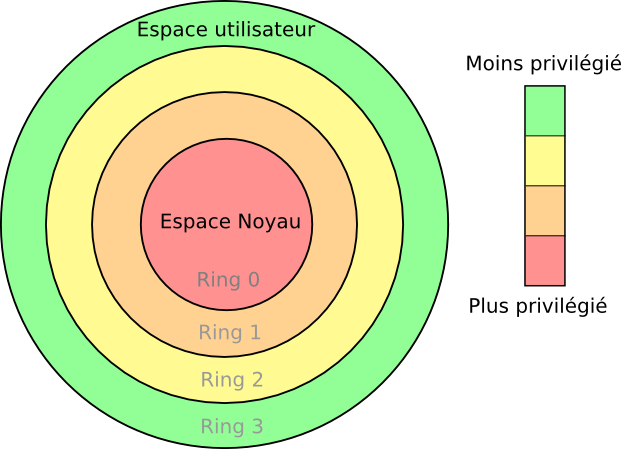
\includegraphics[height=0.5\textheight]{images/Priv_rings.png}
      
      {\tiny Crédit image : \og Hertzsprung \fg{} sur wikipedia, modifié pour le cours}
    \end{center}
  \end{frame}
  
  \begin{frame}
    \frametitle{Les modèles de virtualisation en un schéma}
    \begin{center}
      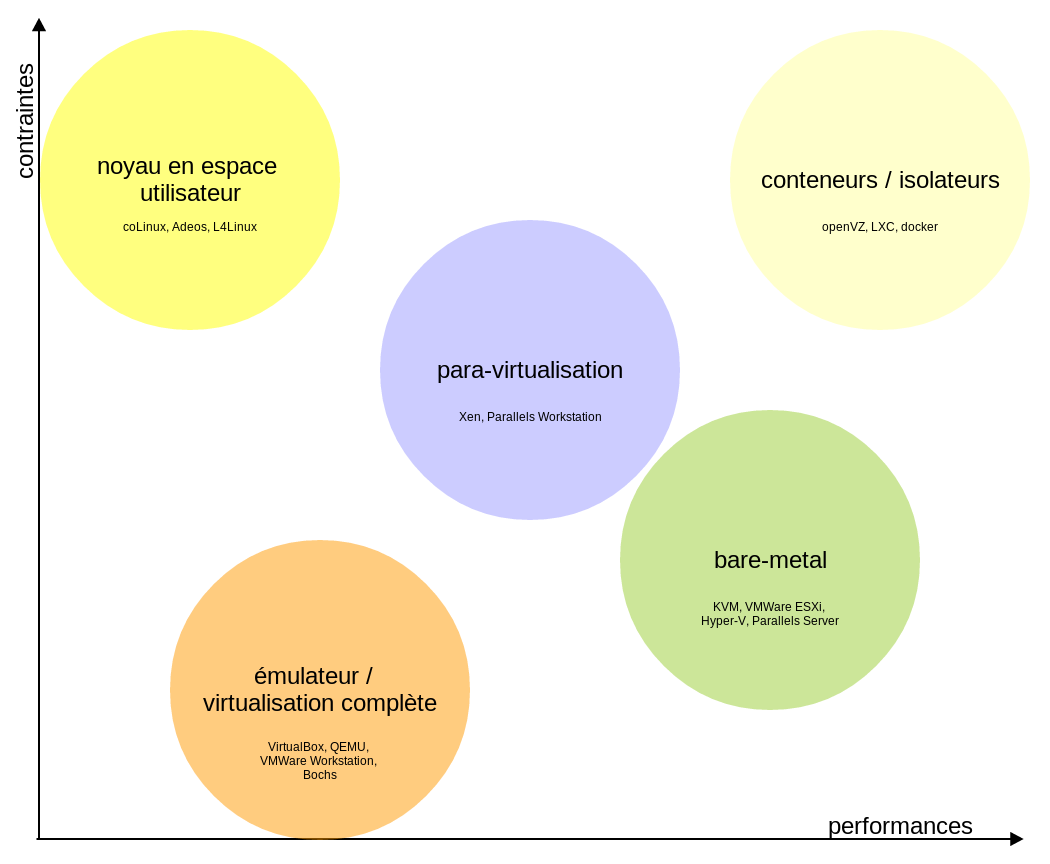
\includegraphics[width=0.8\linewidth]{images/solutions-virtualisation-2.png}
    \end{center}
  \end{frame}
  
  \begin{frame}
    \frametitle{Les conteneurs / isolateurs}
    Principe : isoler l'éxécution d'applications dans un contexte (aussi appelé zone d'éxécution)
    \note{Un peu comme un chroot}
    \begin{itemize}
      \item Pros :
      \begin{itemize}
        \item Très performant car peu d'overhead 
        \item Permet de faire tourner la même application en mode multi-instance (ex: serveur web)
      \end{itemize}
      \item Cons :
      \begin{itemize}
        \item Même noyau pour toutes les applications
        \item Seulement linux
        \item Pas vraiment de la virtualisation
      \end{itemize}
    \end{itemize}
    \begin{center}
      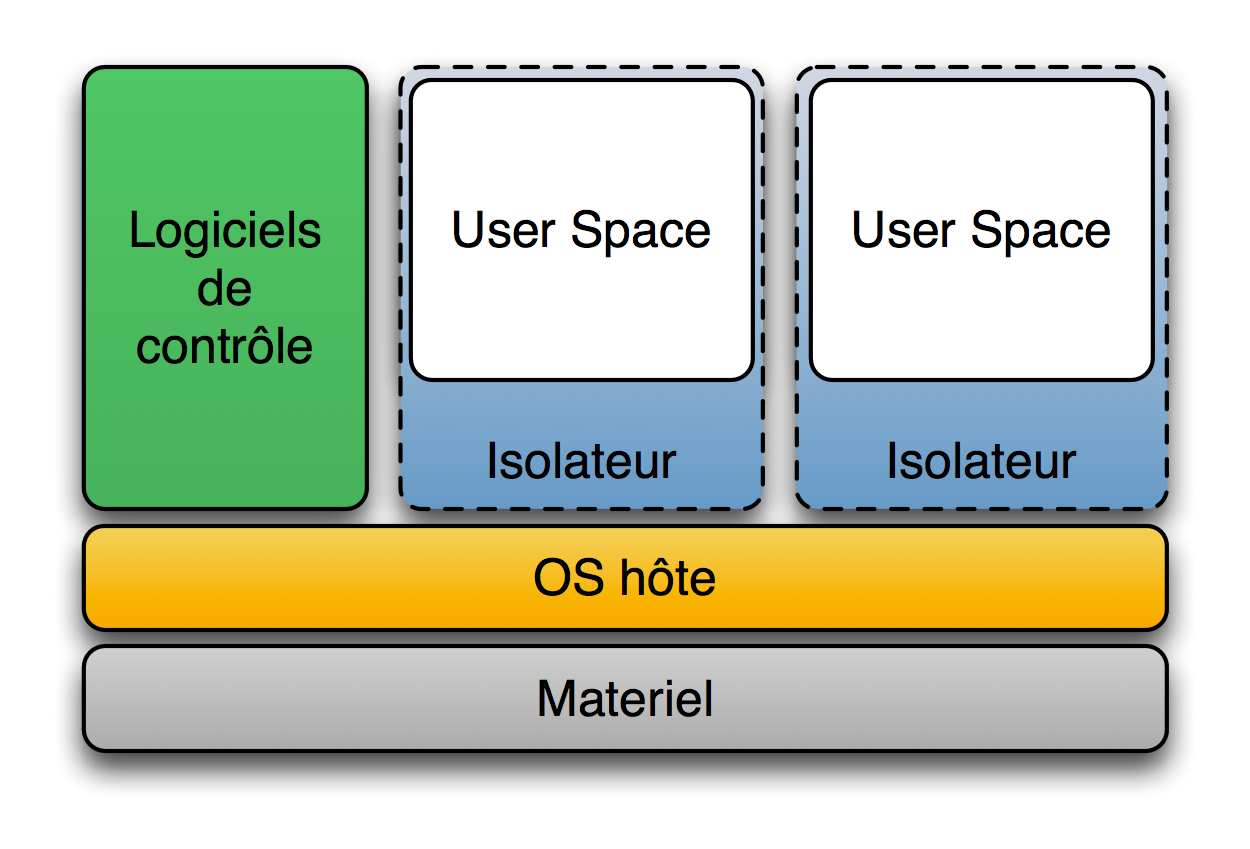
\includegraphics[width=0.5\linewidth]{images/Diagramme_ArchiIsolateur.png}
    \end{center}
  \end{frame}
  
  \begin{frame}
    \frametitle{Noyau en espace utilisateur}
    Principe : faire tourner un noyau Linux dans l'espace utilisateur
    \begin{itemize}
      \item Pros :
      \begin{itemize}
        \item Utile pour tester un noyau linux ou faire du développement de noyau 
      \end{itemize}
      \item Cons :
      \begin{itemize}
        \item Pas très performant (empilement de deux noyaux)
        \item Pas très sécurisé (pas d'isolation entre les noyaux)
        \item Nécessite une modification du noyau invité (possible avec linux seulement)
      \end{itemize}
    \end{itemize}
    \begin{center}
      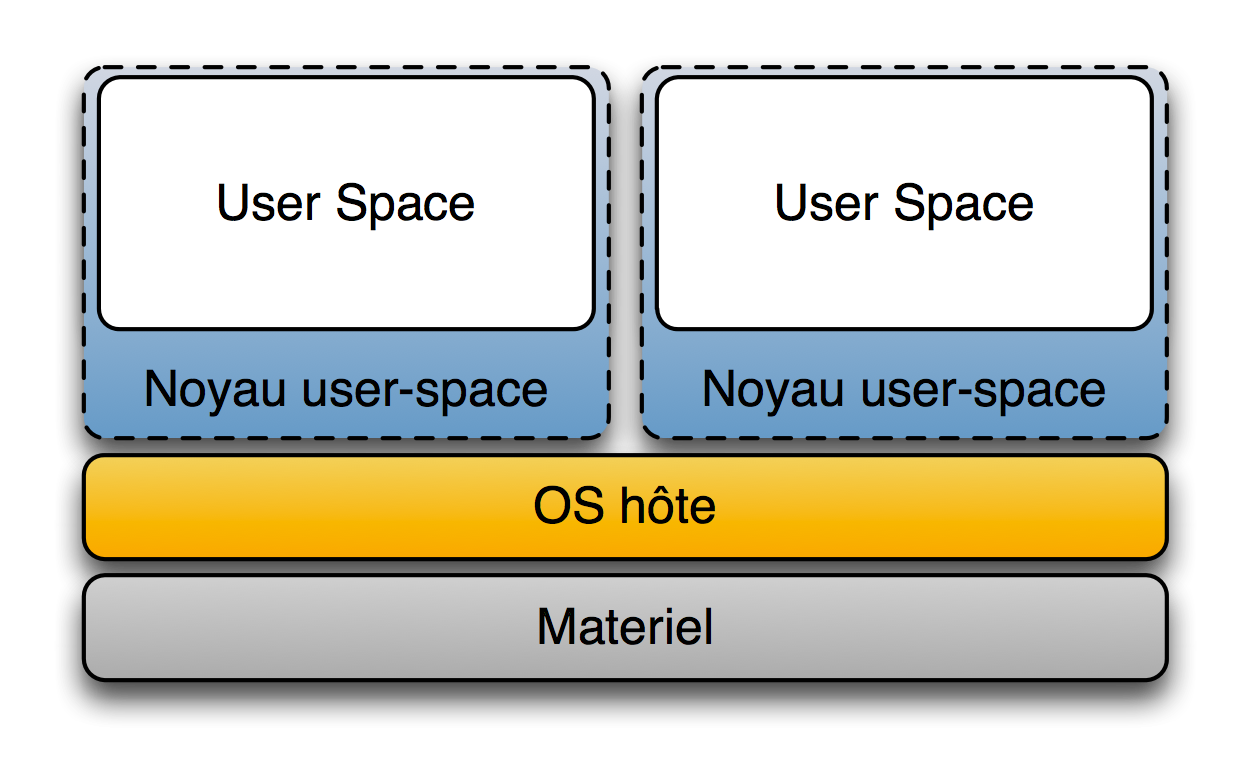
\includegraphics[width=0.5\linewidth]{images/Diagramme_ArchiKernelUserSpace.png}
    \end{center}
  \end{frame}
  
  \begin{frame}
    \frametitle{Émulation / Full virtualisation (Hyperviseur de type 2)}
    Principe : la machine hôte émule le matériel pour la machine invité
    \note{émulateur NES, PS utilisent ce principe là}
    \begin{itemize}
      \item Pros :
      \begin{itemize}
        \item Bonne isolation entre les OS invités
        \item Cohabitation d'architecture CPU et OS hétérogènes
      \end{itemize}
      \item Cons :
      \begin{itemize}
        \item Pas très performant (émulation provoque beaucoup d'overhead)
      \end{itemize}
    \end{itemize}
    \begin{center}
      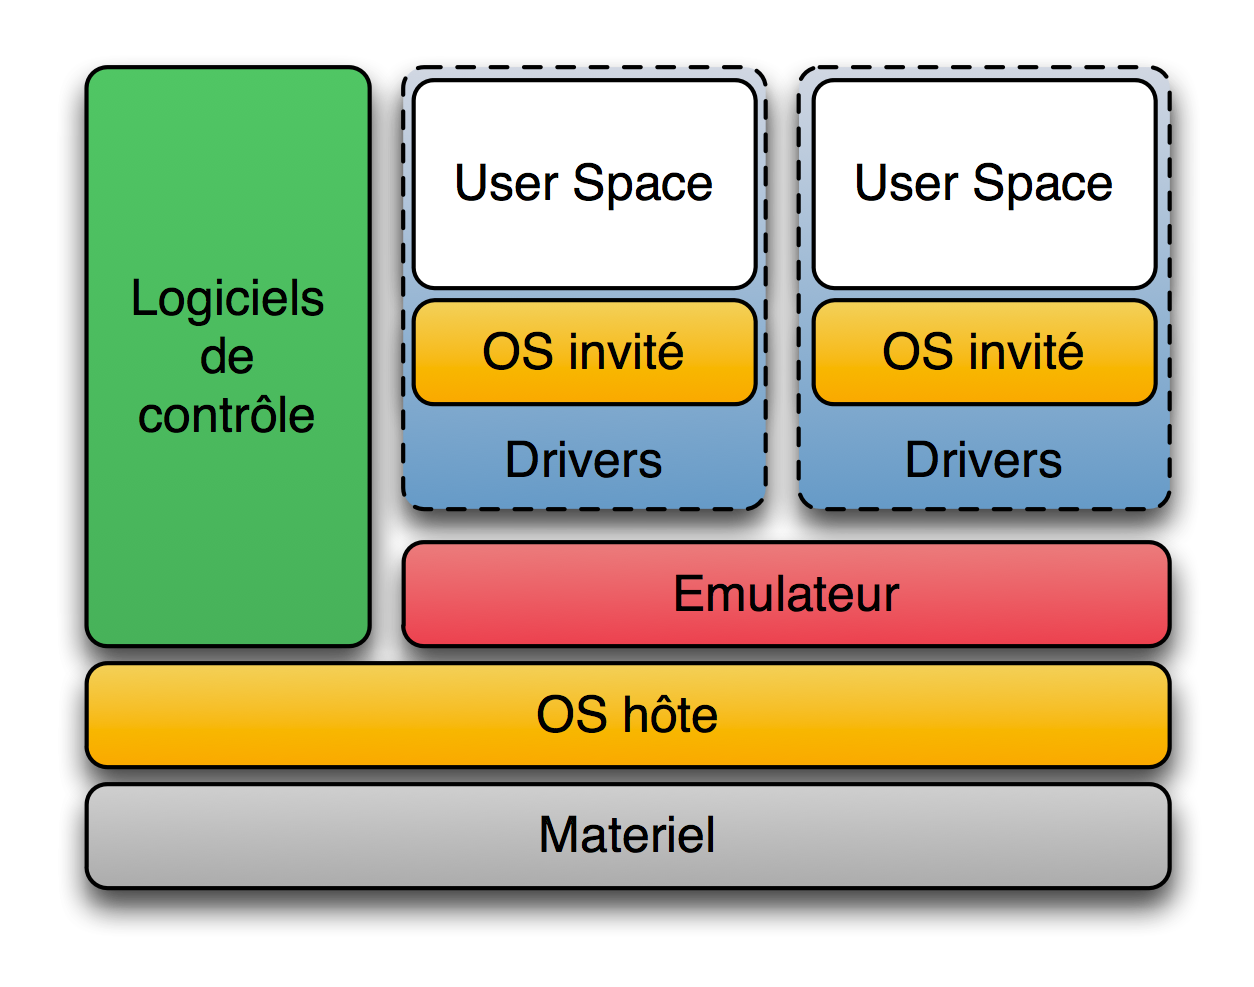
\includegraphics[width=0.5\linewidth]{images/Diagramme_ArchiEmulateur.png}
    \end{center}
  \end{frame}
  
  \begin{frame}
    \frametitle{Para-virtualisation}
    Principe : évolution de l'émulation par modification des OS invités
    \begin{itemize}
      \item Pros :
      \begin{itemize}
        \item Bonne isolation entre les OS invités
        \item Cohabitation d'architecture CPU et OS hétérogènes
        \item Performance correctes
      \end{itemize}
      \item Cons :
      \begin{itemize}
        \item Nécessite la modification du noyau de l'OS invité (possible sur Linux seulement)
      \end{itemize}
    \end{itemize}
    \begin{center}
      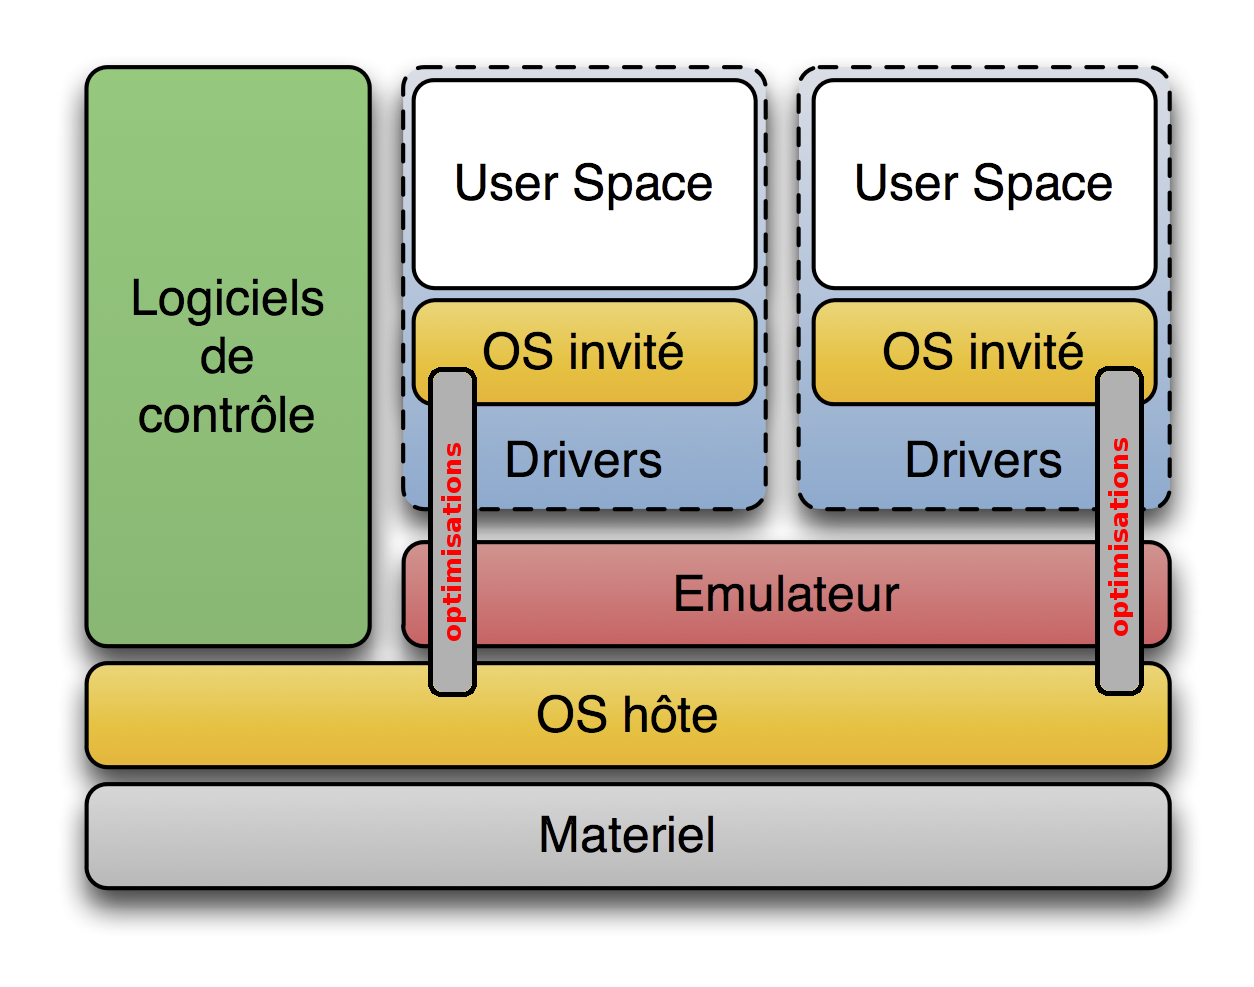
\includegraphics[width=0.5\linewidth]{images/Diagramme_ArchiEmulateur-para.png}
    \end{center}
  \end{frame}
  
  \begin{frame}
    \frametitle{Bare metal (Hyperviseur de type 1)}
    Principe : noyau système léger qui partage l’accès aux ressources matérielles avec les OS invités
    \note{l'hyperviseur de type 1 fait le lien entre les VM et le matériel, il se positionne souvent dans le ring -1, voir slide suivant}
    \begin{itemize}
      \item Pros :
      \begin{itemize}
        \item Bonne isolation entre les OS invités
        \item Cohabitation d'architecture CPU et OS hétérogènes
        \item Très performant (couche d'abstraction minimale)
      \end{itemize}
      \item Cons :
      \begin{itemize}
        \item Nécessite la virtualisation matérielle (Intel VT-x ou AMD-V)
      \end{itemize}
    \end{itemize}
    \begin{center}
      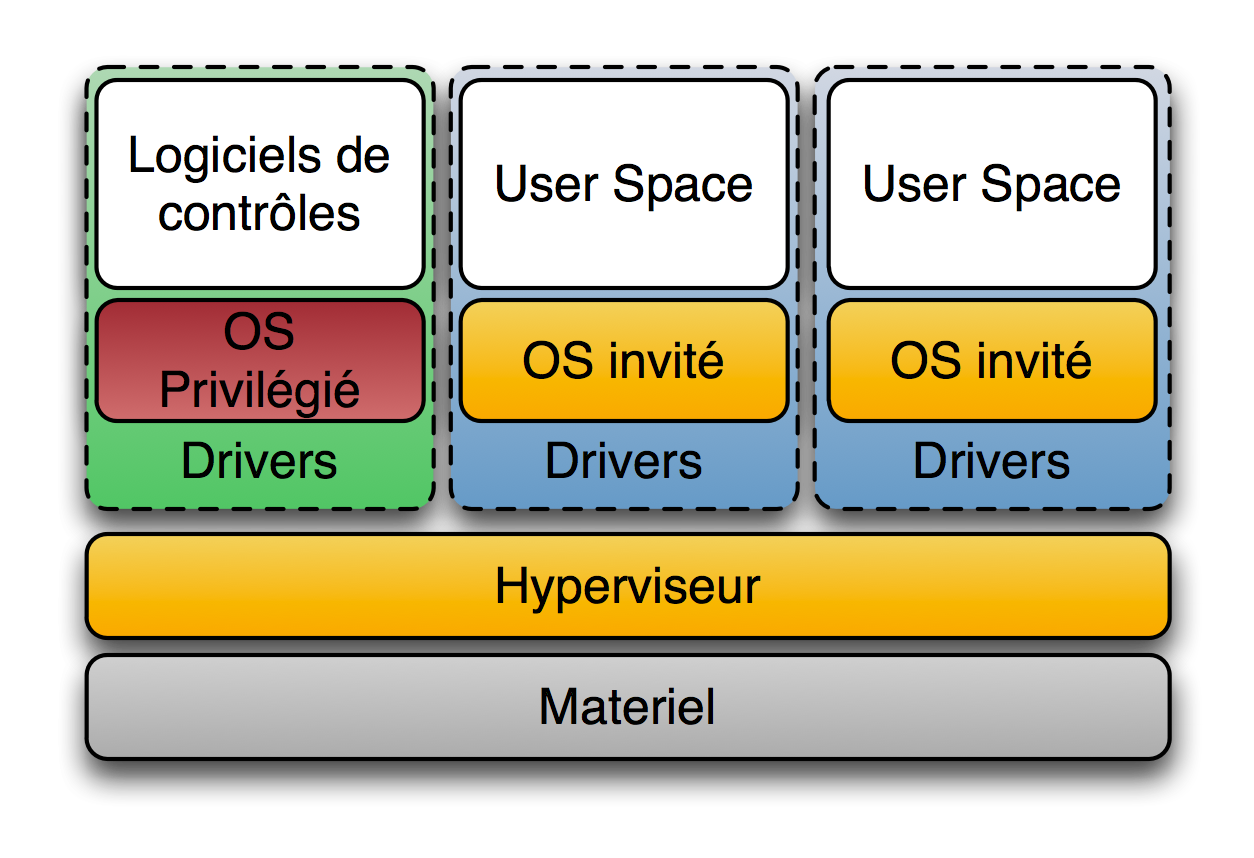
\includegraphics[width=0.5\linewidth]{images/Diagramme_ArchiHyperviseur.png}
    \end{center}
  \end{frame}
  
  \begin{frame}
    \frametitle{Assistance matérielle}
    À partir de 2004, Intel et AMD ont ajouté à leurs processeurs des instructions CPU supplémentaires pour aider à la virtualisation :
    \begin{itemize}
      \item Intel VT-x, VT-c, VT-d
      \item AMD-V
    \end{itemize}
    
    \og To assist virtualization, VT and Pacifica insert a new privilege level beneath Ring 0. Both add nine new machine code instructions that only work at "Ring -1," intended to be used by the hypervisor. \fg{}
  \end{frame}
  
  \begin{frame}
    \frametitle{Démo}
    \huge{Exemples de création de machines virtuelles}
  \end{frame}
